\documentclass[11pt]{beamer}
\usepackage[ngerman]{babel}
\usepackage[utf8]{inputenc}
\usepackage[T1]{fontenc}
\usepackage{lmodern}

\usepackage{multicol}
\usepackage{csquotes}
\usetheme{Singapore}
\begin{document}
	\author{Andreas Windorfer}
	\title{Tango Bäume}
	%\subtitle{}
	%\logo{}
	%\institute{}
	\date{\today}
	%\subject{}
	%\setbeamercovered{transparent}
	%\setbeamertemplate{navigation symbols}{}
	\begin{frame}{}
		\titlepage
	\end{frame}
	\begin{frame} {Übersicht}
		\tableofcontents[]   
		
	\end{frame}
	
	\section{Binärer Suchbaum}
	
	
		\begin{frame} {Binärer Suchbaum}
			\begin{figure}[h]
				\centering
				\includegraphics[width=0.75\textwidth]{"Medien/pres/ioSuchbaum"}
			\end{figure}    
		\end{frame}

			\begin{frame} {Binärer Suchbaum}
			\begin{figure}[h]
				\centering
				\includegraphics[width=0.75\textwidth]{"Medien/pres/suchbaum2_2"}
			\end{figure}    
		\end{frame}

			\begin{frame} {Binärer Suchbaum}
			\begin{figure}[h]
				\centering
				\includegraphics[width=0.75\textwidth]{"Medien/pres/VorgaengerNachfolger"}
			\end{figure}    
		\end{frame}
	
	\begin{frame} {Binärer Suchbaum}
			\begin{figure}[h]
				\centering
				\includegraphics[width=0.75\textwidth]{"Medien/pres/LinksRechtsRotation"}
			\end{figure}    
		\end{frame}	
	
	\section{Dynamische Optimalität}
	
		\begin{frame} {Übersicht}
			\tableofcontents[currentsection]   
		\end{frame}
	
	   
    
    
  \begin{frame} {	\textit{access}$\left(k\right)$ Operation}
    \begin{block}{Parameter / Rückgabe}
    	\begin{itemize}
    		\item Parameter $k$: Schlüssel im BST (Schlüsselmenge $K$)
    		\item Rückgabe: Knoten mit Schlüssel $k$
      \end{itemize}
    			
    \end{block}	
  \end{frame}	
     
     \begin{frame} {	\textit{access}$\left(k\right)$ Operation}
     	\begin{block}{Einschränkungen}
     		Ein Zeiger $p$ (berührter Knoten) in die Struktur:
     		\begin{itemize}
     			\item Setze $p$ auf ein Kind von $p$ 
     			\item Setze $p$ auf den Elternknoten von $p$ 
     			\item Rotationen 
     		\end{itemize}	
     	\end{block}	
     	\pause 
     	\begin{block}{Berechnung der Kosten}
     		
     		Einheitskosten von \enquote{1}.
     	\end{block}	    	
     \end{frame}	    
     
      
  \begin{frame} {	Zugriffsfolgen} 
    \begin{block}{Zugriffsfolgen}
    	\begin{itemize}
    		\item   $X = x_1, x_2,..., x_m$ , mit $\forall i \in \{1,2,..,m\}: x_i \in K$
    		\item  \textit{access}$\left(x_1\right)$,   \textit{access}$\left(x_2\right)$, ....,  
    		\textit{access}$\left(x_m\right)$  
    	\end{itemize}
    \end{block}			
	\pause
   \begin{block}{dynamische BST}
	 \begin{itemize}
		\item Anpassung der Struktur 	 
 	\end{itemize}
   \end{block}			
 \begin{block}{Kostenrechnung}
		\textit{Anzahl der Einzelschritte} + $m$	 
\end{block}		
\end{frame}	  
  \begin{frame} {	dynamisch Optimal} 
	\begin{block}{$\mathit{OPT}\left(X\right)$}
		Niedrigste Kosten zum Ausführen von $X$ 
	\end{block}			
	\pause
	\begin{block}{dynamisch Optimal}
	BST mit Kosten von  $O\left(\mathit{OPT}\left(X\right)\right)$, für beliebige $X$
	\end{block}			
	\begin{block}{c-competitive}
		BST mit Kosten von  $O\left(c \cdot \mathit{OPT}\left(X\right)\right)$, für beliebige $X$	 
	\end{block}		
\end{frame}	  
    
\section{Tango Baum}
	\tableofcontents[]   
 \begin{frame} {Tango Baum} 
 	\begin{block}{Eigenschaten}
 		\begin{itemize}
 			\item 	Aus BSTs bestehender BST
 			\item $\log\left(\log\left(n\right)\right)$-competitive		
 		\end{itemize}
    \end{block}
	\begin{block}{Literatur}
	Erik D. Demaine, Dion. Harmon, John. Iacono, and Mihai. Patrascu.
	Dynamic optimality-almost. SIAM Journal on Computing, 37(1):240
	251, 2007.
    \end{block}
\end{frame}	  
 \begin{frame} {Interleave Lower Bound} 
 	\begin{block}{Motivation}
 	\begin{itemize}
 		\item Berechnung einer unteren Schranke zu $\mathit{OPT\left(X\right)}$
 		\item Beweis der $\log\left( \log \left(n\right)\right)$-competitiveness	
 	\end{itemize}
     \end{block}
\end{frame}	  

 \begin{frame} {Lower Bound Tree} 
	\begin{block}{Definition}
		  Zu $X = x_1,x_2,.,x_m$ und $K = \{k \in \mathbb{N} \vert k \textit{ ist in $X$ enthalten}\}$\\
		  \pause
		  ist der komplette BST $P$ mit der Schlüsselmenge $K$ der LBT. 
		 
	\end{block}
\end{frame}

\begin{frame} {Beispiel LBT} 
\begin{figure}[H]
	\centering
	\includegraphics[width=1\textwidth]{"Medien/pres/lowerBoundTree"}
	\caption{Der Lower Bound Tree zur Zugriffsfolge $1 ,2, .., 14$.  }
	\label{fig:demlowerBoundTree}
\end{figure}
\end{frame}		


 \begin{frame} {Lower Bound Tree} 
	\begin{block}{Linke Region eines Kontens $v$}
	      Schlüssel des linken Teilbaumes von $v$ und \textit{key}$\left(v\right)$	
	\end{block}
    \begin{block}{Linke Region eines Kontens $v$}
	Schlüssel des rechten Teilbaumes von $v$
	\end{block}
	\begin{block}{Interleave durch $v$}
		$x_{i-1}$ liegt in der linken Region und $x_i$ in der rechten,\\
		oder umgekehrt.
    \end{block}
\end{frame}

 \begin{frame} {Lower Bound Tree} 
	\begin{block}{\textit{inScore} $\left(X, v\right)$}
		Anzahl der Interleaves durch $v$
	\end{block}
	\begin{block}{$\mathit{IB}\left(X\right)$}
		$\mathit{IB}\left(X\right) = \sum_{u \in U} \mathit{inScore}\left(X, u\right)$
	\end{block}
\end{frame}

\begin{frame} {Transition Points} 
	$T_0$ Startzustand, $T_i$ nach ausführen von \textit{access} $x_i$.
	\pause
	$j \in {0,1,..m}$\\
	\bigskip
	Zu jedem Knoten $u$ aus $P$, mit nicht leerer rechter Region,\\
	existiert ein transition point in $T_j$ 
	
	
\end{frame}

\begin{frame} {Transition Points} 
	Sei $v$ der Transition Point zu $u$ und $T_j$
	\begin{enumerate}
		\item Im Pfad von der Wurzel zu $v$ ist ein Knoten mit einem Schlüssel aus der linken Region von $u$ enthalten.
		\item Im Pfad von der Wurzel zu $v$ ist ein Knoten mit einem Schlüssel aus der rechten Region von $u$ enthalten.
		\item Kein anderer Knoten mit kleinerer Tiefe erfüllt die Eigenschaften eins und zwei. 
	\end{enumerate}	
\end{frame}
\begin{frame} {Transition Points} 
	Sei $U$ die Menge der Knoten in $P$ mit einer nicht leeren rechten Region.
	\begin{itemize}
		\item Lemma 1: Es gibt zu jedem Knoten $u \in U$ genau einen transition point in $T_j$. 	
		\item Lemma 2: Wird ein transition point nicht berührt, so ist er noch immer der transition point des selben Knotens.
		\item Lemma 3: Ein Knoten kann nicht der transition point mehrerer Knoten sein. 
	\end{itemize}	
\end{frame}

\begin{frame} {Beweis Lemma 1}
\begin{enumerate}
	\item  $l$	ist der kleinste Schlüssel der linken Region
	\item  $r$	ist der größte Schlüssel der rechten Region
	\pause
	\item der Teilbaum mit der Wurzel $u$ enthält genau die Schlüssel aus $K^r_l = \{k \in K \vert k \in \left[l,r\right]\}$
	\pause
	\item  $v_l$ ist der Vorfahre der Schlüssel der linken Region
	\item  $v_r$ ist der Vorfahre der Schlüssel der rechten Region
	\item  $w$ ist der gemeinsame Vorfahre dieser Schlüssel
\end{enumerate}	
\end{frame}

\begin{frame} {Beweis Lemma 1}
\begin{figure}[H]
	\centering
	\includegraphics[width=1\textwidth]{"Medien/pres/linksRechts1"}
\end{figure}
\end{frame}
\begin{frame} {Beweis Lemma 1}
	\begin{figure}[H]
		\centering
		\includegraphics[width=1\textwidth]{"Medien/pres/linksRechts2"}
	\end{figure}
\end{frame}

\begin{frame} {Beweis Lemma 1}
	\begin{enumerate}
			\item  $l$	ist der kleinste Schlüssel der linken Region
		\item  $r$	ist der größte Schlüssel der rechten Region
		\pause
		\item der Teilbaum mit der Wurzel $u$ enthält genau die Schlüssel aus $K^r_l = \{k \in K \vert k \in \left[l,r\right]\}$
		\pause
		\item  $v_l$ ist der Vorfahre der Schlüssel der linken Region
		\item  $v_r$ ist der Vorfahre der Schlüssel der rechten Region
		\item  $w$ ist der gemeinsame Vorfahre dieser Schlüssel
		\item  $w = v_l$ bzw. $w = v_r$	
		\item  Transition point ist $v_r$ bzw. $v_l$ 
	\end{enumerate}	
\end{frame}
\begin{frame} {Transition Point Zuordnung}
	\begin{figure}[H]
		\centering
		\includegraphics[width=1\textwidth]{"Medien/pres/transitionPoints"}
		\caption{Links ein Lower Bound Tree, rechts ein BST }
	\end{figure}
\end{frame}

\begin{frame} {Satz Interleave Lower Bound}
		Sei $X = x_0, x_1,.., x_m$  eine Zugriffsfolge und $n$ die Anzahl der Knoten im zu $X$ erstellten Lower Bound Tree Y. Dann gilt\\	
	$\mathit{OPT}\left(X\right) \geq \mathit{IB}\left(X\right) /2 - n$ .
	
\end{frame}

\begin{frame} {Beweis Interleave Lower Bound}
	\begin{enumerate}
		\item Zählen der Berührungen von Transition Points
		\item Die Anzahl der Berührungen kann für jeden Knoten einzeln bestimmt werden. (Lemma $5.1$ und $5.3$)
		\pause
		\item Betrachteter Knoten $u$. \mbox{$X{^r_l}' = x_{i_0},x_{i_1},..,x_{i_p}$} bilden
		\item $\mathit{inScore}\left(X, u\right) = p$
		\pause
		\item  Sei $q \in \mathbb{N}$ mit $1 \leq q \leq \lfloor p / 2 \rfloor$
		\pause
		\item  Es folgen mindestens $\lfloor p/2 \rfloor \geq p/2 - 1$ Berührungen des transition points von $u$
		\pause
		\item $\mathit{IB}\left(X\right) /2 - \vert U \vert \geq \mathit{IB}\left(X\right) /2 - n$
	\end{enumerate}
	
\end{frame}


\begin{frame} {Aufbau des Tango Baumes}
		\begin{figure}[H]
			\centering
			\includegraphics[width=1\textwidth]{"Medien/pres/tangoBaum"}
		\end{figure}
	Erweiterte Knoten:
	\begin{multicols}{3}
		\begin{enumerate}
			\item \textit{depth}
			\item \textit{minDepth}
			\item \textit{maxDepth}
		\end{enumerate}
	\end{multicols}
\end{frame}

\begin{frame} {Aufbau des Tango Baumes}
	\begin{itemize}
		\item preferred childs
	\end{itemize}
	\begin{figure}[H]
		\centering
		\includegraphics[width=1\textwidth]{"Medien/pres/prefChilds"}
	\end{figure}
\pause
	\begin{itemize}
	\item preferred paths
\end{itemize}
\begin{figure}[H]
	\centering
	\includegraphics[height=0.2\textwidth]{"Medien/pres/prefPaths"}
\end{figure}
\end{frame}


\begin{frame} {Aufbau des Tango Baumes}
		\begin{itemize}
		\item Hilfsbäume
	\end{itemize}
	\begin{figure}[H]
		\centering
		\includegraphics[width=1\textwidth]{"Medien/pres/Hilfsbaeume"}
	\end{figure}
\end{frame}

\begin{frame} {Aufbau des Tango Baumes}
	\begin{figure}[H]
		\centering
		\includegraphics[width=1\textwidth]{"Medien/pres/tangoBaum"}
	\end{figure}
\end{frame}

\begin{frame} {Aufbau des Tango Baumes}
	\begin{itemize}
		\item \textit{access}$\left(9\right)$
	\end{itemize}
	\begin{figure}[H]
		\centering
		\includegraphics[width=1\textwidth]{"Medien/pres/prefChilds"}
	\end{figure}

\end{frame}

\begin{frame} {Aufbau des Tango Baumes}
	\begin{itemize}
		\item \textit{access}$\left(9\right)$
	\end{itemize}
	\begin{figure}[H]
		\centering
		\includegraphics[width=1\textwidth]{"Medien/pres/prefChilds2"}
	\end{figure}
	
\end{frame}



\begin{frame} {Aufbau des Tango Baumes}
		\begin{itemize}
		\item \textit{access}$\left(9\right)$
	\end{itemize}
	\begin{figure}[H]
		\centering
		\includegraphics[width=1\textwidth]{"Medien/pres/tangoBaum2"}
	\end{figure}
\end{frame}


\begin{frame} {\textit{access }Operation}
		\begin{itemize}
		\item Suche findet im HB mit der Tango Baum Wurzel satt.
	\end{itemize}
	
	Anforderungen an die DS der Hilfsbäume
	\begin{enumerate}
		\item $h = O\left(\log\left(n\right)\right)$
		\item \textit{concatenate} ( \textit{HB} $H_1$, \textit{Knoten } $v$, \textit{HB} $H_2$)\\
		Zusammenführen von $T_1$ und $T_2$. Laufzeit $O\left(\log\left(n\right)\right)$
		\item \textit{split} ( \textit{Schlüssel} $k$ )\\
		Zerteilen der eigenen Struktur. Laufzeit $O\left(\log\left(n\right)\right)$
	\end{enumerate}
 \end{frame}

    \begin{frame} { \textit{concatenate} ( \textit{HB} $H_1$, \textit{Knoten } $v$, \textit{HB} $H_2$)}
    	\begin{figure}[H]
    		\centering
    		\includegraphics[width=1\textwidth]{"Medien/pres/concat"}
    	\end{figure}
    \end{frame}

  \begin{frame} {\textit{split} ( \textit{Schlüssel} $k$ )}
	\begin{figure}[H]
		\centering
		\includegraphics[width=1\textwidth]{"Medien/pres/split"}
	\end{figure}
\end{frame}


\begin{frame} {Hilfsoperationen für \textit{access}}
	\begin{enumerate}
		\item\textit{join} (\textit{HB} $T_1$ , \textit{HB} $T_2$)\\
		Vereinigen von $T_1$ und $T_2$
		\item\textit{cut} (\textit{depth} $d$ )\\
		Zerteilen der eigenen Struktur beim Knoten mit Tiefe $d$
	\end{enumerate}
	
\end{frame}

\begin{frame} {\textit{cut} Operation}
	\begin{figure}[H]
		\centering
		\includegraphics[width=1\textwidth]{"Medien/pres/cut"}
	\end{figure}	
\end{frame}
\begin{frame} {\textit{join} Operation}
	\begin{figure}[H]
		\centering
		\includegraphics[width=1\textwidth]{"Medien/pres/join"}
	\end{figure}	
\end{frame}

\begin{frame} {\textit{access} Operation}
	\begin{figure}[H]
		\centering
		\includegraphics[width=1\textwidth]{"Medien/pres/cutJoin"}
	\end{figure}	
\end{frame}


\begin{frame} {Laufzeit von \textit{access}}
	\begin{enumerate}
         \item $\mathit{IB}\left(X\right)$ Interleaves führen zu $\mathit{IB}\left(X\right)$  Wechsel bei preferred children von links nach rechts, oder umgekehrt.
         \item maximal $n$ zusätzliche Wechsel bei preferred children, durch Erstzugriffe in Teilbäume 
         \pause
         \item Das ergibt maximal  $\mathit{IB}\left(X\right) + n$ Wechsel bei preferred children 
         \pause
         \item Es wird maximal $\mathit{IB}\left(X\right) + n + 1$ mal an der Wurzel des Tango Baumes gestartet.
         \item Für die Höhe eines Hilfsbaumes gilt $O\left(\log\left(\log\left(n\right)\right)\right)$
         \pause
         \item $O\left(\left(\mathit{IB}\left(X\right) + n +m \right) \left( 1 + \log \left(\log\left(n\right)\right)\right) \right)$
         \pause
         \item 	$O\left(\left(\mathit{OPT}\left(X\right) + n  \right) \left( 1 + \log \left(\log\left(n\right)\right)\right) \right)$, mit $\mathit{OPT}\left(X\right) \geq \mathit{IB}\left(X\right) /2 -n $
    \end{enumerate} 
\end{frame}

\begin{frame} {Laufzeit von \textit{access}}
	Einzelne Access Operation:
	\begin{enumerate}
		\item $\Theta\left(\log\left(n\right)\right)$ Wechsel bei preferred children
		\pause
		\item $  O \left(\log\left(n\right)   \left( \log \left(\log\left(n\right)\right) + 1\right)\right)$
		\pause
		\item Balancierte BSTs erreichen $O \left( \log\left(n\right)\right)$
	\end{enumerate} 
\end{frame}

\section{Splay Baum}
	\tableofcontents[]   
\begin{frame} {Splay Baum}
	\begin{enumerate}
		\item dynamisch
		\item keine zusätzliche Attribute
		\item kein balancierter BST
		\item $\log \left(n\right)$-competitive bewiesen
		\item dynamische Optimalität vermutet
	\end{enumerate} 
\end{frame}

\begin{frame} {\textit{access}}
	\begin{enumerate}
		\item  \textit{splay} aufrufen
		\item Knoten an der Wurzel zurückgeben
	\end{enumerate}
\end{frame}

\begin{frame} {\textit{access}}
	\begin{enumerate}
		\item  \textit{splay} aufrufen
		\item Knoten an der Wurzel zurückgeben
	\end{enumerate}
\end{frame}
\begin{frame} {\textit{splay}}
	\begin{itemize}
		\item  \textit{zig}
		\item  \textit{zag}
		\item  \textit{zig-zig}
		\item  \textit{zag-zag}
		\item  \textit{zig-zag}
		\item  \textit{zag-zig}
	\end{itemize}
\end{frame}


\begin{frame}{\textit{splay}}
		\begin{figure}[H]
		\centering
		\includegraphics[width=1\textwidth]{"Medien/pres/zigzag"}
	\end{figure}
\end{frame}

\begin{frame}{Eine einzige \textit{splay} Operation}
	\begin{figure}[H]
		\centering
		\includegraphics[width=1\textwidth]{"Medien/pres/splay"}
	
	\end{figure}
	{Daniel Dominic Sleator and Robert Endre Tarjan. Self-adjusting binary
	search trees. J. ACM, 32(3):652-686, July 1985.}
\end{frame}


\begin{frame}{Access Lemma}
	\begin{figure}[H]
		Sei $T$ ein Splay Baum mit $n$ Knoten, Wurzel $w$ und einem Knoten $v$ mit dem Schlüssel $k$. Die amortisierten Kosten von \textit{splay}$\left(k\right)$ sind maximal $3 \left(r\left(w\right) - r\left(v\right)\right) + 1 = O\left(\log\left(\mathit{tw}\left(w\right) / \mathit{tw}\left(v\right)\right) \right) = O\left(\log\left(n\right)\right)$. 
	\end{figure}
\end{frame}

\begin{frame}{Beweis Access Lemma}
	\begin{block}{Potentialfunktionsmethode}
		\begin{itemize}
			\item Gewichtsfunktion $w\left(v\right) \geq 0$ 
			\pause 
			\item $U$ ist Menge der Knoten im Teilbaum mit Wurzel $v$
			\item $\mathit{tw}\left(v\right) = \sum_{u \in U} w\left(u\right)$
			\pause 
			\item Rang $r\left(v\right) = \log_2 \left(tw\left(v\right)\right)$
			\pause
			\item $V$ ist Menge der Knoten im Gesamtbaum
			\item $\Phi = \sum_{v \in V} r\left(v\right)$
		\end{itemize}
	\end{block}
\end{frame}
\begin{frame}{Beweis Access Lemma}
		\begin{figure}[H]
		\centering
		\includegraphics[width=1\textwidth]{"Medien/pres/zigZigKlein"}
		
	\end{figure}
	
	\begin{block}{Kosten Einzelschritt}
		$\leq 3 \left(r\left(v\right)' - r\left(v\right)\right) + 1$
	\end{block}
\end{frame}

\begin{frame}{Beweis Access Lemma}
		\begin{figure}[H]
		\centering
		\includegraphics[width=1\textwidth]{"Medien/pres/zigZigKlein"}
		
	\end{figure}
	\begin{align*}
	& 2 + r\left(u\right)' +r\left(v\right)' +r\left(x\right)' - r\left(u\right)- r\left(v\right)- r\left(x\right)\\
    = & 2 + r\left(u\right)' +r\left(x\right)' - r\left(u\right)- r\left(v\right)\\
     \leq &  2 + r\left(v\right)' + r\left(x\right)' - 2 r\left(v\right) 
	\end{align*}
\end{frame}

\begin{frame}{Beweis Access Lemma}
	\begin{figure}[H]
		\centering
		\includegraphics[width=1\textwidth]{"Medien/pres/zigZigKlein"}
		
	\end{figure}
	\begin{align*}
	&	2 + r\left(v\right)' + r\left(x\right)' - 2 r\left(v\right) \leq  3\left(r\left(v\right)'- r\left(v\right)\right)\\
	\end{align*}
	
\end{frame}

\begin{frame}{Beweis Access Lemma}
	\begin{figure}[H]
		\centering
		\includegraphics[width=1\textwidth]{"Medien/pres/zigZigKlein"}
		
	\end{figure}
	\begin{align*}
	&	2 + r\left(v\right)' + r\left(x\right)' - 2 r\left(v\right) \leq  3\left(r\left(v\right)'- r\left(v\right)\right)\\
	\Leftrightarrow &2 \leq 2r\left(v\right)' -  r\left(x\right)' - r\left(v\right)
	\end{align*}
	
\end{frame}


\begin{frame}{Beweis Access Lemma}
	\begin{figure}[H]
		\centering
		\includegraphics[width=1\textwidth]{"Medien/pres/zigZigKlein"}
		
	\end{figure}
	\begin{align*}
	&	2 + r\left(v\right)' + r\left(x\right)' - 2 r\left(v\right) \leq  3\left(r\left(v\right)'- r\left(v\right)\right)\\	
	\Leftrightarrow &2 \leq 2r\left(v\right)' -  r\left(x\right)' - r\left(v\right)\\
	\Leftrightarrow & -2 \geq -2r\left(v\right)' +  r\left(x\right)' + r\left(v\right)
	\end{align*}
	
\end{frame}


\begin{frame}{Beweis Access Lemma}
	\begin{figure}[H]
		\centering
		\includegraphics[width=1\textwidth]{"Medien/pres/zigZigKlein"}
		
	\end{figure}
    \begin{align*}
         &	2 + r\left(v\right)' + r\left(x\right)' - 2 r\left(v\right) \leq  3\left(r\left(v\right)'- r\left(v\right)\right)\\       
        \Leftrightarrow &2 \leq 2r\left(v\right)' -  r\left(x\right)' - r\left(v\right)\\
         \Leftrightarrow & -2 \geq -2r\left(v\right)' +  r\left(x\right)' + r\left(v\right)\\
        \Leftrightarrow & -2 \geq \log_2\left(\mathit{tw}\left(x'\right) / \mathit{tw}\left(v'\right)\right) +   \log_2\left(\mathit{tw}\left(v\right) / \mathit{tw}\left(v'\right)\right)
    \end{align*}
	
\end{frame}
\begin{frame}{Beweis Access Lemma}
	\begin{figure}[H]
		\centering
		\includegraphics[width=1\textwidth]{"Medien/pres/zigZigKlein"}
		
	\end{figure}

	$-2 \geq \log_2\left(\mathit{tw}\left(x'\right) / \mathit{tw}\left(v'\right)\right) +   \log_2\left(\mathit{tw}\left(v\right) / \mathit{tw}\left(v'\right)\right)$\\
	 \bigskip

	 Für $a,b \in \mathit{R}$ mit $a,b > 0$ und $a + b \leq 1$ gilt: $\log_2\left(a\right) + \log_2\left(b\right) \leq -2$
\end{frame}
\begin{frame}{Beweis Access Lemma}
	\begin{figure}[H]
		\centering
		\includegraphics[width=1\textwidth]{"Medien/pres/zigZigKlein"}
		
	\end{figure}
	
	$-2 \geq \log_2\left(\mathit{tw}\left(x'\right) / \mathit{tw}\left(v'\right)\right) +   \log_2\left(\mathit{tw}\left(v\right) / \mathit{tw}\left(v'\right)\right)$\\
	\bigskip
	
	Für $a,b \in \mathit{R}$ mit $a,b > 0$ und $a + b \leq 1$ gilt: $\log_2\left(a\right) + \log_2\left(b\right) \leq -2$
\end{frame}
\begin{frame}{Beweis Access Lemma}
		\begin{align*}
		&	3(r'(v) - r(v) ) + 3(r''(v) - r'(v)) + 3(r'''(v) - r''(v))...  + 1 \\
		= & 3 (r(w) - 3r(v))  + 1 
	\end{align*}
\end{frame}


\section{Laufzeittests}
	\tableofcontents[]   
	\begin{frame}{Zufällig erzeugte Zugriffsfolgen.}
		\begin{center}
				$m = 40.000.000$\\
		\end{center}
		\begin{figure}[H]
			\centering
			\includegraphics[width=1\textwidth]{"Medien/pres/randomAccess1"}
			\caption{Beste Zeiten des Tango Baumes.}
		\end{figure}
	\end{frame}

\begin{frame}{Zufällig erzeugte Zugriffsfolgen}
	\begin{figure}[H]
		\centering
		\includegraphics[width=1\textwidth]{"Medien/pres/randomAccess2"}
		\caption{Beste Zeiten des Splay Baumes.}
	\end{figure}
\end{frame}

\begin{frame}{Zufällig erzeugte Zugriffsfolgen}
		\begin{figure}[H]
		\centering
		\includegraphics[width=1\textwidth]{"Medien/pres/randomAccess3"}
		\caption{Durchschnittliche Werte.}
	\end{figure}
\end{frame}


\begin{frame}{Auffälligkeiten}
	\begin{enumerate}
	\item Tango Kennlinie zu Durchschnittswerten
	\item Große Differenzen zwischen Tango- und Splay Baum 
	\end{enumerate}
\end{frame}



\begin{frame}{Tango Kennlinie}
	\begin{table}
		\begin{center}
			Durchschnittswerte $n = 10.000$
			\begin{tabular}[c]{|l|l|l|}
				\hline
				$i$ & Zeit Tango $\left(s\right)$ &Zeit Splay $\left(s\right)$\\
				\hline
				$1$ & $354$ &$16$ \\
				\hline
				$2$ & $841$ &$21$ \\
				\hline
				$3$ & $345$ &$15$  \\
				\hline
				$4$ & $819$ &$31$ \\
				\hline
				$5$ & $352$ &$15$  \\
				\hline
				$6$ & $344$ &$16$  \\
				\hline		
				$7$ & $334$ &$16$ \\
				\hline
				$8$ & $329$ &$16$ \\
				\hline
				$9$ & $328$ &$15$  \\
				\hline
				$10$ & $332$ &$16$  \\
				\hline
				avg & $438$  & $18$	\\
				\hline
			\end{tabular}
		\end{center}
	\end{table}
\end{frame}


\begin{frame}{Dynamic Finger Property}
	\begin{itemize}
		\item $X = x_i, x_2,.., x_m$
		\item $K = \{1,2,..,n\}$
	\end{itemize}
     \begin{block}{Definition}
     	\begin{align*}
     	O\left( m + n + \sum_{i = 2}^{m} \log \left(\vert x_{i-1} - x_i  \vert	+ 1	\right)\right)
     	\end{align*} 
     \end{block}
\end{frame}

\begin{frame}{Dynamic Finger Property}
	Splay Baum: ja \\
	Richard Cole, Bud Mishra, Jeanette Schmidt, and Alan Siegel. On the
	dynamic finger conjecture for splay trees. part i: Splay sorting log n-block
	sequences. SIAM Journal on Computing,  2000.\\
	\bigskip
	\bigskip
	Tango Baum: nein
	
	
\end{frame}

\begin{frame}{Dynamic Finger Property}
     Zugriffsfolgen der Form:  $1, 3, 5,..,n-1, n-3, n-5, ..,1, 3, 5..., n-1,...$ 
     
	\begin{figure}[H]
		\centering
		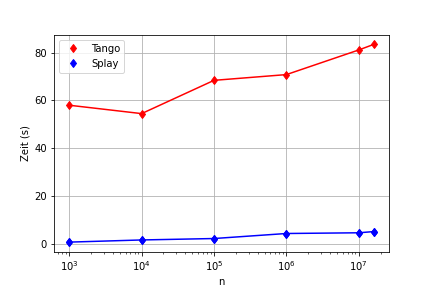
\includegraphics[width=0.7\textwidth]{Medien/pres/dynamicfinger}
	\end{figure}
\end{frame}
\begin{frame}{Dynamic Finger Property}
	Zugriffsfolgen der Form:  $1, 3, 5,..,n-1, n-3, n-5, ..,1, 3, 5..., n-1,...$ 
	
	\begin{figure}[H]
		\centering
		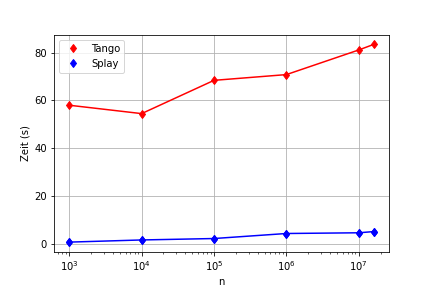
\includegraphics[width=0.7\textwidth]{Medien/pres/dynamicfinger}
	\end{figure}
\end{frame}

\begin{frame} {Dynamic Finger Property}
\begin{table}[H]
	\begin{center}
		\begin{tabular}[c]{|c|c|c|}
			\hline
			$n$ & Zeit Tango in $\left(s\right)$ &Zeit Splay in $\left(s\right)$ \\
			\hline
			$10^3$ & $58$ &$0,8$ \\
			\hline
			$10^4$  & $54,5$ &$1,7$  \\
			\hline
			$10^5$  & $68,4$ &$2,3$  \\
			\hline
			$10^6$  & $70,8$ &$4,4$  \\
			\hline
			$10^7$  & $81,1$ &$4,7$  \\
			\hline
			$1,6 *10^7$  & $83,3$ &$5,2$  \\
			\hline
		\end{tabular} 
	\end{center}
\end{table}	
\end{frame}
\begin{frame}
	\begin{center}
			Vielen Dank für Ihre Aufmerksamkeit
	\end{center}

\end{frame}

\end{document}